Bradley and Dunlop written two works about BVI navigation, one in \citeyear{bradley2002investigating} and the last in \citeyear{bradley2005experimental}. 

\subsection{The 2002 investigation}

On 2002 they studied which information BVI users used throughout their navigation and compared the data collected with another similar data, but instead it was answered by sighted users. This second data was also collected by the same researchers in a prior investigation, made also in 2002, and both of the data were collected using the same interview's structure.

This investigation was made by analysing the answers from a interview with the participants. In this interview, the participants had to explain how to arrive to two different location as if they were talking to someone with the same condition. The answer were than classified in 11 different categories:

\begin{itemize}
    \item Directional (e.g. left/right, north/south)
    \item Structural (e.g. road, monument, church)
    \item Environmental (e.g. hill, river, tree)
    \item Textual-structural (e.g. name of shops, places, restaurants)
    \item Textual-area/street based (e.g. name of street, neighborhoods, squares)
    \item Numerical (e.g. first, second, 100m)
    \item Descriptive (e.g. steep, tall)
    \item Temporal/Distance based (e.g. \textit{"walk until you reach..."} or \textit{"before you get to"})
    \item Sensory (e.g. sound of engines, smell of bread from a bakery)
    \item Motion (e.g. cars passing by, doors opening)
    \item Social Contact (e.g. asking people or using a guide dog for help)
\end{itemize}

The motion and the social contact was added in the interview with the BVI users, so the researches re-analysed the sighted answers to fill this classification as well. The Figures \ref{fig:bradley_2002} and \ref{fig:bradley_2002_2} show their findings.

\begin{figure}[!htb]
    \centering
    \tikzstyle{barraVI} = [fill = cor1]
    \tikzstyle{barraS} = [fill = cor2]
    \tikzstyle{legenda} = [fill = white, line width = 0.25mm]
    \tikzstyle{--} = [line width = 0.25mm]
    
    \resizebox{0.8\linewidth}{!}{
    \begin{tikzpicture}[node distance=0cm]
        % Fundo do gráfico
    
        \renewcommand{\tamX}{13.875cm}
        \renewcommand{\tamY}{5.4cm}
        
        \node (origin) {};
        \node (endX) [xshift = \tamX] {};
        \node (endY) [yshift = \tamY] {};
        \node (endXY) [above of = endX, yshift = \tamY] {};
        
        %Título
        \node (titulo) [xshift = \tamX*0.5, yshift = \tamY + 1.25cm] {\textbf{Average nº of utterances used within each contextual category}}
        node [below of = titulo, yshift = -0.5cm] {\textbf{between sighted and visually impaired participants}};
        
        \draw[--] (origin.west) node[anchor = east]{\footnotesize 0} to (endX.center) node[anchor = north, xshift = -7.5cm, yshift = -2.0cm]{\textbf{Type of contextual categories}};
        \draw[--] (origin.south) to (endY.center) node[anchor = east, xshift = -1.0cm,rotate = 90]{\textbf{Average nº of utterance}};
        \draw[--] (endX.center) to (endXY.center);
        
        \foreach \r/\n in        {1/5,2/10,3/15,4/20,5/25,6/30,7/35,8/40,9/45,10/50,11/55,12/60,13/65,14/70,15/75,16/80,17/85,18/90}
        {
            \draw [--] (-0.15,0.30cm*\r) node[anchor = east]{\footnotesize \n} to (\tamX,0.30cm*\r);
        }
        
        \renewcommand{\largX}{0.25}
        \renewcommand{\altY}{0}
        \renewcommand{\distX}{0.5}
        %Direct
        \draw[barraVI] (\distX,0) node[yshift = -1.0cm, rotate = 45]{Direct} rectangle ++(\largX,5.3);
        \draw[barraS] (\distX+\largX,0) rectangle ++(\largX,1.6);
        \draw[--] (\distX+3.5*\largX,0) to ++(0,-0.2);
        
        \renewcommand{\distX}{1.75}
        %Struct
        \draw[barraVI] (\distX,0) node[yshift = -1.0cm, rotate = 45]{Struct} rectangle ++(\largX,3.6);
        \draw[barraS] (\distX+\largX,0) rectangle ++(\largX,0.5);
        \draw[--] (\distX+3.5*\largX,0) to ++(0,-0.2);
        
        \renewcommand{\distX}{3.0}
        %Struct
        \draw[barraVI] (\distX,0) node[yshift = -1.0cm, rotate = 45]{Environ} rectangle ++(\largX,0.5);
        \draw[barraS] (\distX+\largX,0) rectangle ++(\largX,0.2);
        \draw[--] (\distX+3.5*\largX,0) to ++(0,-0.2);
        
        \renewcommand{\distX}{4.25}
        %Struct
        \draw[barraVI] (\distX,0) node[yshift = -1.0cm, rotate = 45]{Text-struct} rectangle ++(\largX,0.2);
        \draw[barraS] (\distX+\largX,0) rectangle ++(\largX,0.4);
        \draw[--] (\distX+3.5*\largX,0) to ++(0,-0.2);
        
        \renewcommand{\distX}{5.5}
        %Struct
        \draw[barraVI] (\distX,0) node[yshift = -1.0cm, rotate = 45]{Text-area/st} rectangle ++(\largX,0.5);
        \draw[barraS] (\distX+\largX,0) rectangle ++(\largX,0.7);
        \draw[--] (\distX+3.5*\largX,0) to ++(0,-0.2);
        
        \renewcommand{\distX}{6.75}
        %Struct
        \draw[barraVI] (\distX,0) node[yshift = -1.0cm, rotate = 45]{Numer} rectangle ++(\largX,1.3);
        \draw[barraS] (\distX+\largX,0) rectangle ++(\largX,0.2);
        \draw[--] (\distX+3.5*\largX,0) to ++(0,-0.2);
        
        \renewcommand{\distX}{8.0}
        %Struct
        \draw[barraVI] (\distX,0) node[yshift = -1.0cm, rotate = 45]{Desc} rectangle ++(\largX, 4.2);
        \draw[barraS] (\distX+\largX,0) rectangle ++(\largX,0.45);
        \draw[--] (\distX+3.5*\largX,0) to ++(0,-0.2);
        
        \renewcommand{\distX}{9.25}
        %Struct
        \draw[barraVI] (\distX,0) node[yshift = -1.0cm, rotate = 45]{Sensory} rectangle ++(\largX,0.8);
        \draw[barraS] (\distX+\largX,0) rectangle ++(\largX,0.0);
        \draw[--] (\distX+3.5*\largX,0) to ++(0,-0.2);
        
        \renewcommand{\distX}{10.5}
        %Struct
        \draw[barraVI] (\distX,0) node[yshift = -1.0cm, rotate = 45]{Tem/Dist} rectangle ++(\largX,0.95);
        \draw[barraS] (\distX+\largX,0) rectangle ++(\largX,0.35);
        \draw[--] (\distX+3.5*\largX,0) to ++(0,-0.2);
        
        \renewcommand{\distX}{11.75}
        %Struct
        \draw[barraVI] (\distX,0) node[yshift = -1.0cm, rotate = 45]{Motion} rectangle ++(\largX,0.1);
        \draw[barraS] (\distX+\largX,0) rectangle ++(\largX,0.0);
        \draw[--] (\distX+3.5*\largX,0) to ++(0,-0.2);
        
        \renewcommand{\distX}{13.0}
        %Struct
        \draw[barraVI] (\distX,0) node[yshift = -1.0cm, rotate = 45]{Social} rectangle ++(\largX,0.2);
        \draw[barraS] (\distX+\largX,0) rectangle ++(\largX,0.0);
        \draw[--] (\distX+3.5*\largX,0) to ++(0,-0.2);
        
        %Legenda
        \draw[legenda] (\tamX-3.0cm,\tamY-1.5cm) rectangle (\tamX+1.5cm, \tamY+0.25cm);
        \draw[barraVI] (\tamX-2.5cm,\tamY-0.25cm) rectangle ++(0.25cm,0.25cm) node[anchor = west, xshift = 0.15cm, yshift = -0.15cm]{Visualy Impaired};
        \draw[barraS] (\tamX-2.5cm,\tamY-1.0cm) rectangle ++(0.25cm,0.25cm) node[anchor = west, xshift = 0.15cm, yshift = -0.15cm]{Sighted};
        
    \end{tikzpicture}
    }
    \centering
    \caption{Comparison between sighted participants with BVI participants (Adapted from \citeonline{bradley2002investigating}).}
    \label{fig:bradley_2002}
\end{figure}

\begin{figure}[!htb]
    \centering
    
    \tikzstyle{barraVI} = [fill = cor1]
    \tikzstyle{barraS} = [fill = cor2]
    \tikzstyle{legenda} = [fill = white, line width = 0.25mm]
    \tikzstyle{--} = [line width = 0.25mm]
    
    \resizebox{0.8\linewidth}{!}{
    \begin{tikzpicture}[node distance=0cm]
        % Fundo do gráfico
    
        \renewcommand{\tamX}{11cm}
        \renewcommand{\tamY}{4.5cm}
        
        \node (origin) {};
        \node (endX) [xshift = \tamX] {};
        \node (endY) [yshift = \tamY] {};
        \node (endXY) [above of = endX, yshift = \tamY] {};
        
        %Título
        \node (titulo) [xshift = \tamX*0.5, yshift = \tamY + 1.25cm] {\textbf{Average nº of contextual categories used per participant}}
        node [below of = titulo, yshift = -0.5cm] {\textbf{within sighted and visually impaired groups}};
        
        
        % Eixos
        \draw[--] (origin.west) node[anchor = north, yshift = -0.25cm]{\footnotesize 0} to (endX.center)
        node[anchor = north, xshift = -5.5cm, yshift = -1.0cm]{\textbf{Average nº of categories used for each route description}};
        \draw[--] (origin.south) to (endY.center) 
        node(eixoY)[anchor = east, xshift = -5.0cm, yshift = -0.5cm, rotate = 90]{\textbf{Groups used for}}
        node[right of = eixoY, xshift = 0.5cm, rotate = 90] {\textbf{comparison}};
        \draw[--] (endX.center) to (endXY.center);
        
        \foreach \r in {1,2,...,11}
        {
            \draw [--] (1cm*\r,0) node[anchor = north, yshift = -0.25cm]{\footnotesize \r} to (1cm*\r, \tamY);
        }
        
        \renewcommand{\largY}{0.75}
        \renewcommand{\altY}{0}
        \renewcommand{\distY}{0.75}
        
        
        %Sighted
        \draw[barraS] (0,\distY) node[xshift = -1.0cm, yshift = 0.35cm]{Sighted} rectangle ++(6.3cm,\largY);
        \draw[--] (0,(\distY+2.0*\largY) to ++(-0.2,0);
        %\draw[barraS] (\distX+\largX,0) rectangle ++(\largX,1.6);
        
        \renewcommand{\distY}{3.0}
        %Visually Impaired
        \draw[barraVI] (0,\distY) node[xshift = -2.0cm, yshift = 0.35cm]{Visually Impaired} rectangle ++(9.7cm,\largY);
        \draw[--] (0,(\distY+2.0*\largY) to ++(-0.2,0);
        
    \end{tikzpicture}
    }
    \centering
    \caption{Number of categories used by each group \cite{bradley2002investigating}.}
    \label{fig:bradley_2002_2}
\end{figure}

In conclusion the researches realised that BVI participants use less text-based information than the sighted participants, but BVI participants used more words to describe a path than the sighted participants.

Besides describing the paths to reach the destinations, the researches also asked the BVI participants their "opinions on the importance of different types of contextual information for route navigation, design issues relating to usability and their mobile needs/requirements" \cite{bradley2002investigating}. Many participants said that white canes and guide dogs had limitations and also commented that sensory information are very important when different types were used together in order to confirm one information. 

\subsection{The 2005 experiment}

Based on the findings from 2002, Bradley and Dunlop designed an experiment to investigate if there is a difference between the perceived workload of both BVI participant and sighted participants when then navigate using a user-tailored information created with the results of both previous experiments.

16 participants, 8 sighted and 8 BVI, were recruited to walk to four pre-determined landmarks at the centre of Glasgow. They followed the same orientations that were pre-recorded and given to the participants. For each participant, orientations for 2 of these 4 landmarks, that were made using based on the proportions of the results of the sighted users' interview, were randomly given. Similar was made with the remaining 2 landmarks, but with orientations made with the findings of the BVI users' interview. These proportions are presented at the Table \ref{tab:bradley_2005_table}

\begin{table}[htbp]
    \centering
    \caption{Proportion of each type of information used by sighted and BVI participants \cite{bradley2005experimental}}
    \begin{tabular}{|l|l|l|}
        \hline
        \textbf{Class of contextual information} & \textbf{\% Used Sighted} & \textbf{\% Used BVI} \\ \hline
        1. Directional                           & 37.4                     & 30.1                 \\ \hline
        2. Structural                            & 11.5                     & 20.1                 \\ \hline
        3. Environmental                         & 1.6                      & 2.9                  \\ \hline
        4. Textual-structural                    & 9.9                      & 1.2                  \\ \hline
        5. Textual-area/street                   & 15.6                     & 2.7                  \\ \hline
        6. Numerical                             & 5.0                      & 7.5                  \\ \hline
        7. Descriptive                           & 10.8                     & 23.8                 \\ \hline
        8. Temporal/distance                     & 8.2                      & 5.1                  \\ \hline
        9. Sensory                               & 0                        & 4.4                  \\ \hline
        10. Motion                               & 0                        & 0.8                  \\ \hline
        11. Social contact                       & 0                        & 1.4                  \\ \hline
    \end{tabular}
    \label{tab:bradley_2005_table}
\end{table}

Their results found out that BVI users reached landmarks significantly quicker when given the information that were made for that group, but still longer than sighted users. This comparison is show in the Figure \ref{fig:bradley_2005} and \ref{fig:bradley_2005_2}. Condition 1 is the verbal orientation made for sighted users and condition 2 is the verbal orientation made for BVI users

\begin{figure}[htbp]
\centering
\begin{minipage}{.45\linewidth}
    \centering
    \resizebox{\linewidth}{!}{
    \tikzstyle{barraVI} = [fill = cor1]
\tikzstyle{barraS} = [fill = cor2]
\tikzstyle{legenda} = [fill = white, line width = 0.25mm]
\tikzstyle{--} = [line width = 0.25mm]

%\resizebox{0.8\linewidth}{!}{
\begin{tikzpicture}[node distance=0cm]
    % Fundo do gráfico

    \renewcommand{\tamX}{8.0cm}
    \renewcommand{\tamY}{6.0cm}
    
    \node (origin) {};
    \node (endX) [xshift = \tamX] {};
    \node (endY) [yshift = \tamY] {};
    \node (endXY) [above of = endX, yshift = \tamY] {};
    
    %Título
    \node (titulo) [xshift = \tamX*0.5, yshift = \tamY + 1.25cm] {\textbf{\Large Comparing condition times for}}
    node [below of = titulo, yshift = -0.5cm] {\textbf{\Large visually impaired participants}};
    
    \draw[--] (origin.west) node[anchor = east]{\Large 0} to (endX.center) node[anchor = north, xshift = -7.5cm, yshift = -2.0cm]{};
    \draw[--] (origin.south) to (endY.center) node[anchor = east, xshift = -1.5cm,rotate = 90]{\textbf{\Large Average time (secs)}};
    \draw[--] (endX.center) to (endXY.center);
    
   \foreach \r/\n in {1/50,2/100,3/150,4/200,5/250,6/300}
    {
        \draw [--] (-0.15,1cm*\r) node[anchor = east]{\n} to (\tamX,1cm*\r);
    }
    
    \renewcommand{\largX}{0.5}
    \renewcommand{\altY}{0}
    \renewcommand{\distX}{0.5}
    %Direct
    \draw[barraVI] (\distX,0) node[xshift = \largX*1cm, yshift = -0.5cm]{\textbf{\Large Lan 1}} rectangle ++(\largX,4.6);
    \draw[barraS] (\distX+\largX,0) rectangle ++(\largX,4.5);
    \draw[--] (\distX+3*\largX,0) to ++(0,-0.2);
    
    \renewcommand{\distX}{2.5}
    %Struct
    \draw[barraVI] (\distX,0) node[xshift = \largX*1cm, yshift = -0.5cm]{\textbf{\Large Lan 2}} rectangle ++(\largX,5.2);
    \draw[barraS] (\distX+\largX,0) rectangle ++(\largX,5.1);
    \draw[--] (\distX+3*\largX,0) to ++(0,-0.2);
    
    \renewcommand{\distX}{4.5}
    %Struct
    \draw[barraVI] (\distX,0) node[xshift = \largX*1cm, yshift = -0.5cm]{\textbf{\Large Lan 3}} rectangle ++(\largX,4.2);
    \draw[barraS] (\distX+\largX,0) rectangle ++(\largX,4.1);
    \draw[--] (\distX+3*\largX,0) to ++(0,-0.2);
    
    \renewcommand{\distX}{6.5}
    %Struct
    \draw[barraVI] (\distX,0) node[xshift = \largX*1cm, yshift = -0.5cm]{\textbf{\Large Lan 4}} rectangle ++(\largX,5.2);
    \draw[barraS] (\distX+\largX,0) rectangle ++(\largX,5.1);
    \draw[--] (\distX+3*\largX,0) to ++(0,-0.2);
    
    
    %Legenda
    \draw[legenda] (\tamX,\tamY-1.5cm) rectangle ++(2.5cm,2cm);
    \draw[barraVI] (\tamX+0.25cm,\tamY-0.25cm) rectangle ++(0.25cm,0.25cm) 
    node[anchor = west, xshift = 0.15cm, yshift = -0.15cm]{\Large Con 1};
    \draw[barraS] (\tamX+0.25cm,\tamY-1.0cm) rectangle ++(0.25cm,0.25cm) 
    node[anchor = west, xshift = 0.15cm, yshift = -0.15cm]{\Large Con 2};
    
\end{tikzpicture}
%}
    }
    \captionof{figure}{Mean times for each landmark performed by the sighted participants \cite{bradley2005experimental}.}
    \label{fig:bradley_2005}
\end{minipage}
\begin{minipage}{.1\linewidth}
\end{minipage}
\begin{minipage}{.45\linewidth}
    \centering
    \resizebox{\linewidth}{!}{
    \tikzstyle{barraVI} = [fill = cor1]
\tikzstyle{barraS} = [fill = cor2]
\tikzstyle{legenda} = [fill = white, line width = 0.25mm]
\tikzstyle{--} = [line width = 0.25mm]
    
%\resizebox{0.8\linewidth}{!}{
\begin{tikzpicture}[node distance=0cm]
    % Fundo do gráfico

    \renewcommand{\tamX}{8.0cm}
    \renewcommand{\tamY}{6.0cm}
    
    \node (origin) {};
    \node (endX) [xshift = \tamX] {};
    \node (endY) [yshift = \tamY] {};
    \node (endXY) [above of = endX, yshift = \tamY] {};
    
    %Título
    \node (titulo) [xshift = \tamX*0.5, yshift = \tamY + 1.25cm] {\textbf{\Large Comparing condition times for}}
    node [below of = titulo, yshift = -0.5cm] {\textbf{\Large sighted participants}};
    
    \draw[--] (origin.west) node[anchor = east]{\Large 0} to (endX.center) node[anchor = north, xshift = -7.5cm, yshift = -2.0cm]{};
    \draw[--] (origin.south) to (endY.center) node[anchor = east, xshift = -1.5cm, rotate = 90]{\textbf{\Large Average time (secs)}};
    \draw[--] (endX.center) to (endXY.center);
    
   \foreach \r/\n in {1/50,2/100,3/150,4/200,5/250,6/300}
    {
        \draw [--] (-0.15,1cm*\r) node[anchor = east]{\Large \n} to (\tamX,1cm*\r);
    }
    
    \renewcommand{\largX}{0.5}
    \renewcommand{\altY}{0}
    \renewcommand{\distX}{0.5}
    %Direct
    \draw[barraVI] (\distX,0) node[xshift = \largX*1cm, yshift = -0.5cm]{\textbf{\Large Lan 1}} rectangle ++(\largX,3.8);
    \draw[barraS] (\distX+\largX,0) rectangle ++(\largX,3.9);
    \draw[--] (\distX+3*\largX,0) to ++(0,-0.2);
    
    \renewcommand{\distX}{2.5}
    %Struct
    \draw[barraVI] (\distX,0) node[xshift = \largX*1cm, yshift = -0.5cm]{\textbf{\Large Lan 2}} rectangle ++(\largX,4.8);
    \draw[barraS] (\distX+\largX,0) rectangle ++(\largX,4.7);
    \draw[--] (\distX+3*\largX,0) to ++(0,-0.2);
    
    \renewcommand{\distX}{4.5}
    %Struct
    \draw[barraVI] (\distX,0) node[xshift = \largX*1cm, yshift = -0.5cm]{\textbf{\Large Lan 3}} rectangle ++(\largX,3.7);
    \draw[barraS] (\distX+\largX,0) rectangle ++(\largX,3.7);
    \draw[--] (\distX+3*\largX,0) to ++(0,-0.2);
    
    \renewcommand{\distX}{6.5}
    %Struct
    \draw[barraVI] (\distX,0) node[xshift = \largX*1cm, yshift = -0.5cm]{\textbf{\Large Lan 4}} rectangle ++(\largX,4.2);
    \draw[barraS] (\distX+\largX,0) rectangle ++(\largX,4.3);
    \draw[--] (\distX+3*\largX,0) to ++(0,-0.2);
    
    
    %Legenda
    \draw[legenda] (\tamX,\tamY-1.5cm) rectangle ++(2.5cm,2cm);
    \draw[barraVI] (\tamX+0.25cm,\tamY-0.25cm) rectangle ++(0.25cm,0.25cm) 
    node[anchor = west, xshift = 0.15cm, yshift = -0.15cm]{\Large Con 1};
    \draw[barraS] (\tamX+0.25cm,\tamY-1.0cm) rectangle ++(0.25cm,0.25cm) 
    node[anchor = west, xshift = 0.15cm, yshift = -0.15cm]{\Large Con 2};
    
\end{tikzpicture}
%}
    }
    \captionof{figure}{Mean times for each landmark performed by the BVI participants \cite{bradley2005experimental}.}
    \label{fig:bradley_2005_2}
\end{minipage}
\end{figure}

%\begin{figure}[htbp]
%\centering
%\begin{minipage}{.4\linewidth}
%    \centering
%    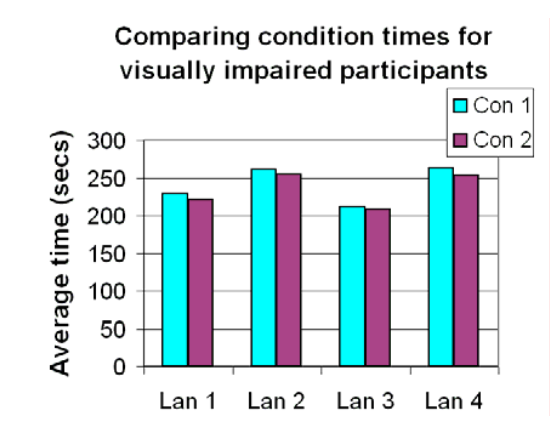
\includegraphics[width=\linewidth]{Revisao/Bradley Dunlop/Bradley Dunlop 2005.png}
%    \vspace{0.1cm}
%    \captionof{figure}{Mean times for each landmark performed by the sighted participants \cite{bradley2005experimental}.}
%    \label{fig:bradley_2005}
%\end{minipage}
%\begin{minipage}{.2\linewidth}
%\end{minipage}
%\begin{minipage}{.4\linewidth}
%    \centering
%    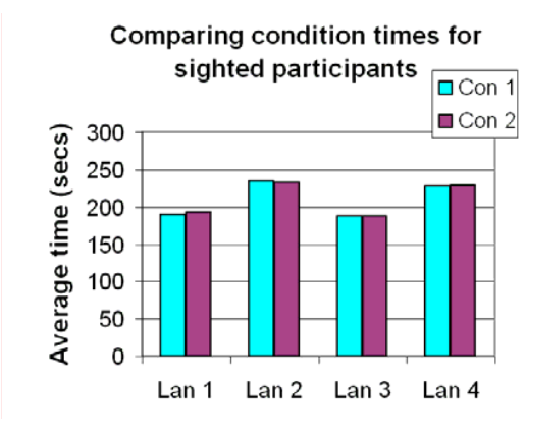
\includegraphics[width=\linewidth]{Revisao/Bradley Dunlop/Bradley Dunlop 2005 (2).png}
%    \captionof{figure}{Mean times for each landmark performed by the BVI participants \cite{bradley2005experimental}.}
%    \label{fig:bradley_2005_2}
%\end{minipage}
%\end{figure}

After the experiment a NASA-TLX was completed by each participant. The score for each dimensions is show in the Figures \ref{fig:bradley_2005_condition} and \ref{fig:bradley_2005_participants}. These scores show that BVI participants did had higher workload when guided by the condition 1 as well as the sighted participants did with the condition 2.

\begin{figure}[htbp]
    \centering
    \begin{subfigure}{.45\textwidth}
        \centering
        \resizebox{1.1\linewidth}{!}{
        \tikzstyle{barraVI} = [fill = cor1]
\tikzstyle{barraS} = [fill = cor2]
\tikzstyle{legenda} = [fill = white, line width = 0.25mm]
\tikzstyle{--} = [line width = 0.25mm]

%\resizebox{0.8\linewidth}{!}{
\begin{tikzpicture}[node distance=0cm]
    % Fundo do gráfico

    \renewcommand{\tamX}{12.0cm}
    \renewcommand{\tamY}{7.0cm}
    
    \node (origin) {};
    \node (endX) [xshift = \tamX] {};
    \node (endY) [yshift = \tamY] {};
    \node (endXY) [above of = endX, yshift = \tamY] {};
    
    %Título
    \node (titulo) [xshift = \tamX*0.5, yshift = \tamY + 2cm] {\textbf{\LARGE Comparing visually impaired}}
    node(titulo2) [below of = titulo, yshift = -0.5cm] {\textbf{\LARGE participants' workload rating for both}}
    node [below of = titulo2, yshift = -0.5cm] {\textbf{\LARGE conditions}};
    
    \draw[--] (origin.west) node[anchor = east]{\Large 0} to (endX.center) node[anchor = north, xshift = -\tamX*0.5, yshift = -1.0cm]{\textbf{\LARGE Type of contextual categories}};
    \draw[--] (origin.south) to (endY.center) 
    node(eixoY)[anchor = east, xshift = -2.5cm, yshift = -0.5cm, rotate = 90]{\textbf{\LARGE Average weighted}}
    node[below of = eixoY, xshift = 0.75cm, rotate = 90] {\textbf{\LARGE score}};
    \draw[--] (endX.center) to (endXY.center);
    
   \foreach \r/\n in {1/50,2/100,3/150,4/200,5/250,6/300, 7/350}
    {
        \draw [--] (-0.15,1cm*\r) node[anchor = east]{\Large \n} to (\tamX,1cm*\r);
    }
    
    \renewcommand{\largX}{0.5}
    \renewcommand{\altY}{0}
    \renewcommand{\distX}{0.5}
    
    %Mental Demand
    \draw[barraVI] (\distX,0) node[xshift = \largX*1cm, yshift = -0.5cm]{\textbf{\LARGE MD}} rectangle ++(\largX,6.1);
    \draw[barraS] (\distX+\largX,0) rectangle ++(\largX,5.7);
    \draw[--] (\distX+3*\largX,0) to ++(0,-0.2);
    
    \renewcommand{\distX}{2.5}
    %Physical Demand
    \draw[barraVI] (\distX,0) node[xshift = \largX*1cm, yshift = -0.5cm]{\textbf{\LARGE PD}} rectangle ++(\largX,0.2);
    \draw[barraS] (\distX+\largX,0) rectangle ++(\largX,0.8);
    \draw[--] (\distX+3*\largX,0) to ++(0,-0.2);
    
    \renewcommand{\distX}{4.5}
    %Temporal demand
    \draw[barraVI] (\distX,0) node[xshift = \largX*1cm, yshift = -0.5cm]{\textbf{\LARGE TD}} rectangle ++(\largX,0.9);
    \draw[barraS] (\distX+\largX,0) rectangle ++(\largX,0.8);
    \draw[--] (\distX+3*\largX,0) to ++(0,-0.2);
    
    \renewcommand{\distX}{6.5}
    %Performance
    \draw[barraVI] (\distX,0) node[xshift = \largX*1cm, yshift = -0.5cm]{\textbf{\LARGE OP}} rectangle ++(\largX,2.2);
    \draw[barraS] (\distX+\largX,0) rectangle ++(\largX,2.1);
    \draw[--] (\distX+3*\largX,0) to ++(0,-0.2);
    
    \renewcommand{\distX}{8.5}
    %Effort
    \draw[barraVI] (\distX,0) node[xshift = \largX*1cm, yshift = -0.5cm]{\textbf{\LARGE EF}} rectangle ++(\largX,4.1);
    \draw[barraS] (\distX+\largX,0) rectangle ++(\largX,3.8);
    \draw[--] (\distX+3*\largX,0) to ++(0,-0.2);
    
    \renewcommand{\distX}{10.5}
    %Frustation
    \draw[barraVI] (\distX,0) node[xshift = \largX*1cm, yshift = -0.5cm]{\textbf{\LARGE FR}} rectangle ++(\largX,3.7);
    \draw[barraS] (\distX+\largX,0) rectangle ++(\largX,1.5);
    \draw[--] (\distX+3*\largX,0) to ++(0,-0.2);
    
    
    %Legenda
    \draw[legenda] (\tamX-2.0cm,\tamY-1.5cm) rectangle ++(4.5cm,2cm);
    \draw[barraVI] (\tamX-1.75cm,\tamY-0.25cm) rectangle ++(0.25cm,0.25cm) 
    node[anchor = west, xshift = 0.15cm, yshift = -0.15cm]{\LARGE Condition 1};
    \draw[barraS] (\tamX-1.75cm,\tamY-1.0cm) rectangle ++(0.25cm,0.25cm) 
    node[anchor = west, xshift = 0.15cm, yshift = -0.15cm]{\LARGE Condition 2};
    
\end{tikzpicture}
%}
        }
        \caption{BVI participants.}
        \label{fig:bradley_2005_condition_1}
    \end{subfigure}
    \hfill
    \begin{subfigure}{.45\textwidth}
        \centering
        \resizebox{1.1\linewidth}{!}{
        \tikzstyle{barraVI} = [fill = cor1]
\tikzstyle{barraS} = [fill = cor2]
\tikzstyle{legenda} = [fill = white, line width = 0.25mm]
\tikzstyle{--} = [line width = 0.25mm]

%\resizebox{0.8\linewidth}{!}{
\begin{tikzpicture}[node distance=0cm]
    % Fundo do gráfico

    \renewcommand{\tamX}{12.0cm}
    \renewcommand{\tamY}{9.0cm}
    
    \node (origin) {};
    \node (endX) [xshift = \tamX] {};
    \node (endY) [yshift = \tamY] {};
    \node (endXY) [above of = endX, yshift = \tamY] {};
    
    %Título
    \node (titulo) [xshift = \tamX*0.5, yshift = \tamY + 2cm] {\textbf{\LARGE Comparing visually impaired}}
    node(titulo2) [below of = titulo, yshift = -0.5cm] {\textbf{\LARGE participants' workload rating for both}}
    node [below of = titulo2, yshift = -0.5cm] {\textbf{\LARGE conditions}};
    
    \draw[--] (origin.west) node[anchor = east]{\Large 0} to (endX.center) node[anchor = north, xshift = -\tamX*0.5, yshift = -1.0cm]{\textbf{\LARGE Type of contextual categories}};
    \draw[--] (origin.south) to (endY.center) 
    node(eixoY)[anchor = east, xshift = -2.5cm, yshift = -0.5cm, rotate = 90]{\textbf{\LARGE Average weighted}}
    node[below of = eixoY, xshift = 0.75cm, rotate = 90] {\textbf{\LARGE score}};
    \draw[--] (endX.center) to (endXY.center);
    
   \foreach \r/\n in {1/20,2/40,3/60,4/80,5/100,6/120, 7/140, 8/160, 9/180}
    {
        \draw [--] (-0.15,1cm*\r) node[anchor = east]{\Large \n} to (\tamX,1cm*\r);
    }
    
    \renewcommand{\largX}{0.5}
    \renewcommand{\altY}{0}
    \renewcommand{\distX}{0.5}
    
    %Mental Demand
    \draw[barraVI] (\distX,0) node[xshift = \largX*1cm, yshift = -0.5cm]{\textbf{\LARGE MD}} rectangle ++(\largX,6.9);
    \draw[barraS] (\distX+\largX,0) rectangle ++(\largX,7.9);
    \draw[--] (\distX+3*\largX,0) to ++(0,-0.2);
    
    \renewcommand{\distX}{2.5}
    %Physical Demand
    \draw[barraVI] (\distX,0) node[xshift = \largX*1cm, yshift = -0.5cm]{\textbf{\LARGE PD}} rectangle ++(\largX,1.3);
    \draw[barraS] (\distX+\largX,0) rectangle ++(\largX,1.2);
    \draw[--] (\distX+3*\largX,0) to ++(0,-0.2);
    
    \renewcommand{\distX}{4.5}
    %Temporal demand
    \draw[barraVI] (\distX,0) node[xshift = \largX*1cm, yshift = -0.5cm]{\textbf{\LARGE TD}} rectangle ++(\largX,1.7);
    \draw[barraS] (\distX+\largX,0) rectangle ++(\largX,1.9);
    \draw[--] (\distX+3*\largX,0) to ++(0,-0.2);
    
    \renewcommand{\distX}{6.5}
    %Performance
    \draw[barraVI] (\distX,0) node[xshift = \largX*1cm, yshift = -0.5cm]{\textbf{\LARGE OP}} rectangle ++(\largX,1.6);
    \draw[barraS] (\distX+\largX,0) rectangle ++(\largX,2.0);
    \draw[--] (\distX+3*\largX,0) to ++(0,-0.2);
    
    \renewcommand{\distX}{8.5}
    %Effort
    \draw[barraVI] (\distX,0) node[xshift = \largX*1cm, yshift = -0.5cm]{\textbf{\LARGE EF}} rectangle ++(\largX,5.9);
    \draw[barraS] (\distX+\largX,0) rectangle ++(\largX,6.2);
    \draw[--] (\distX+3*\largX,0) to ++(0,-0.2);
    
    \renewcommand{\distX}{10.5}
    %Frustation
    \draw[barraVI] (\distX,0) node[xshift = \largX*1cm, yshift = -0.5cm]{\textbf{\LARGE FR}} rectangle ++(\largX,0.3);
    \draw[barraS] (\distX+\largX,0) rectangle ++(\largX,2.8);
    \draw[--] (\distX+3*\largX,0) to ++(0,-0.2);
    
    
    %Legenda
    \draw[legenda] (\tamX-2.0cm,\tamY-1.5cm) rectangle ++(4.5cm,2cm);
    \draw[barraVI] (\tamX-1.75cm,\tamY-0.25cm) rectangle ++(0.25cm,0.25cm) 
    node[anchor = west, xshift = 0.15cm, yshift = -0.15cm]{\LARGE Condition 1};
    \draw[barraS] (\tamX-1.75cm,\tamY-1.0cm) rectangle ++(0.25cm,0.25cm) 
    node[anchor = west, xshift = 0.15cm, yshift = -0.15cm]{\LARGE Condition 2};
    
\end{tikzpicture}
%}
        }
        \caption{Sighted participants}
        \label{fig:bradley_2005_condition_2}
    \end{subfigure}
\caption{Comparison of the NASA-TLX between the conditions \cite{bradley2005experimental}.}
\label{fig:bradley_2005_condition}
\end{figure}

%\begin{figure}[htbp]
%    \centering
%    \begin{subfigure}{.45\textwidth}
%        \centering
%        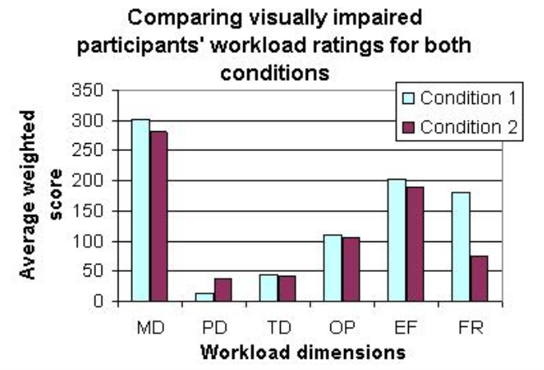
\includegraphics[width=\textwidth]{Revisao/Bradley Dunlop/Bradley Dunlop 2005 Nasa 1.png}
%        \caption{BVI participants.}
%        \label{fig:bradley_2005_condition_1}
%    \end{subfigure}
%    \hfill
%    \begin{subfigure}{.45\textwidth}
%        \centering
%        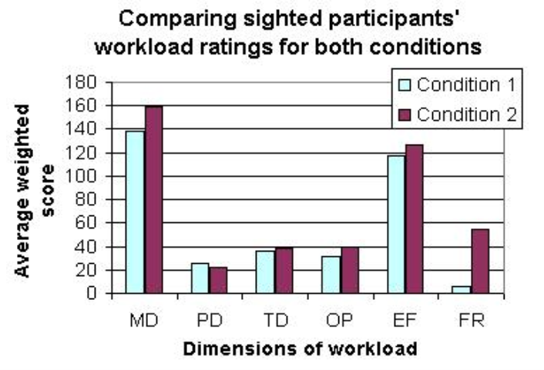
\includegraphics[width=\textwidth]{Revisao/Bradley Dunlop/Bradley Dunlop 2005 Nasa 2.png}
%        \caption{Sighted participants}
%        \label{fig:bradley_2005_condition_2}
%    \end{subfigure}
%\caption{Comparison of the NASA-TLX between the conditions \cite{bradley2005experimental}.}
%\label{fig:bradley_2005_condition}
%\end{figure}


\begin{figure}[htbp]
    \centering
    \begin{subfigure}{.49\textwidth}
        \centering
        \resizebox{\linewidth}{!}{
        \tikzstyle{barraVI} = [fill = cor1]
\tikzstyle{barraS} = [fill = cor2]
\tikzstyle{legenda} = [fill = white, line width = 0.25mm]
\tikzstyle{--} = [line width = 0.25mm]

%\resizebox{0.8\linewidth}{!}{
\begin{tikzpicture}[node distance=0cm]
    % Fundo do gráfico

    \renewcommand{\tamX}{12.0cm}
    \renewcommand{\tamY}{7.0cm}
    
    \node (origin) {};
    \node (endX) [xshift = \tamX] {};
    \node (endY) [yshift = \tamY] {};
    \node (endXY) [above of = endX, yshift = \tamY] {};
    
    %Título
    \node (titulo) [xshift = \tamX*0.5, yshift = \tamY + 1cm] {\textbf{\LARGE Comparing group scores for condition 1}};
    \draw[--] (origin.west) node[anchor = east]{\Large 0} to (endX.center) node[anchor = north, xshift = -\tamX*0.5, yshift = -1.0cm]{\textbf{\LARGE Workload dimensions}};
    \draw[--] (origin.south) to (endY.center) 
    node(eixoY)[anchor = east, xshift = -2.5cm, yshift = 0.5cm, rotate = 90]{\textbf{\LARGE Average weighted score}};
    \draw[--] (endX.center) to (endXY.center);
    
   \foreach \r/\n in {1/50,2/100,3/150,4/200,5/250,6/300, 7/350}
    {
        \draw [--] (-0.15,1cm*\r) node[anchor = east]{\Large \n} to (\tamX,1cm*\r);
    }
    
    \renewcommand{\largX}{0.5}
    \renewcommand{\altY}{0}
    \renewcommand{\distX}{0.5}
    
    %Mental Demand
    \draw[barraVI] (\distX,0) node[xshift = \largX*1cm, yshift = -0.5cm]{\textbf{\LARGE MD}} rectangle ++(\largX,6.1);
    \draw[barraS] (\distX+\largX,0) rectangle ++(\largX,2.8);
    \draw[--] (\distX+3*\largX,0) to ++(0,-0.2);
    
    \renewcommand{\distX}{2.5}
    %Physical Demand
    \draw[barraVI] (\distX,0) node[xshift = \largX*1cm, yshift = -0.5cm]{\textbf{\LARGE PD}} rectangle ++(\largX,0.3);
    \draw[barraS] (\distX+\largX,0) rectangle ++(\largX,0.5);
    \draw[--] (\distX+3*\largX,0) to ++(0,-0.2);
    
    \renewcommand{\distX}{4.5}
    %Temporal demand
    \draw[barraVI] (\distX,0) node[xshift = \largX*1cm, yshift = -0.5cm]{\textbf{\LARGE TD}} rectangle ++(\largX,0.9);
    \draw[barraS] (\distX+\largX,0) rectangle ++(\largX,0.7);
    \draw[--] (\distX+3*\largX,0) to ++(0,-0.2);
    
    \renewcommand{\distX}{6.5}
    %Performance
    \draw[barraVI] (\distX,0) node[xshift = \largX*1cm, yshift = -0.5cm]{\textbf{\LARGE OP}} rectangle ++(\largX,2.2);
    \draw[barraS] (\distX+\largX,0) rectangle ++(\largX,0.6);
    \draw[--] (\distX+3*\largX,0) to ++(0,-0.2);
    
    \renewcommand{\distX}{8.5}
    %Effort
    \draw[barraVI] (\distX,0) node[xshift = \largX*1cm, yshift = -0.5cm]{\textbf{\LARGE EF}} rectangle ++(\largX,4.1);
    \draw[barraS] (\distX+\largX,0) rectangle ++(\largX,2.3);
    \draw[--] (\distX+3*\largX,0) to ++(0,-0.2);
    
    \renewcommand{\distX}{10.5}
    %Frustation
    \draw[barraVI] (\distX,0) node[xshift = \largX*1cm, yshift = -0.5cm]{\textbf{\LARGE FR}} rectangle ++(\largX,3.7);
    \draw[barraS] (\distX+\largX,0) rectangle ++(\largX,0.2);
    \draw[--] (\distX+3*\largX,0) to ++(0,-0.2);
    
    
    %Legenda
    \draw[legenda] (\tamX-3.0cm,\tamY-1.5cm) rectangle ++(6.5cm,2cm);
    \draw[barraVI] (\tamX-2.75cm,\tamY-0.25cm) rectangle ++(0.25cm,0.25cm) 
    node[anchor = west, xshift = 0.15cm, yshift = -0.15cm]{\LARGE Visually impaired};
    \draw[barraS] (\tamX-2.75cm,\tamY-1.0cm) rectangle ++(0.25cm,0.25cm) 
    node[anchor = west, xshift = 0.15cm, yshift = -0.15cm]{\LARGE Sighted};
    
\end{tikzpicture}
%}
        }
        \caption{Condition 1.}
        \label{fig:bradley_2005_nasa_participants_1}
    \end{subfigure}
    \hfill
    \begin{subfigure}{.49\textwidth}
        \centering
        \resizebox{\linewidth}{!}{
        \tikzstyle{barraVI} = [fill = cor1]
\tikzstyle{barraS} = [fill = cor2]
\tikzstyle{legenda} = [fill = white, line width = 0.25mm]
\tikzstyle{--} = [line width = 0.25mm]

%\resizebox{0.8\linewidth}{!}{
\begin{tikzpicture}[node distance=0cm]
    % Fundo do gráfico

    \renewcommand{\tamX}{12.0cm}
    \renewcommand{\tamY}{6.0cm}
    
    \node (origin) {};
    \node (endX) [xshift = \tamX] {};
    \node (endY) [yshift = \tamY] {};
    \node (endXY) [above of = endX, yshift = \tamY] {};
    
    %Título
    \node (titulo) [xshift = \tamX*0.5, yshift = \tamY + 1cm] {\textbf{\LARGE Orientation from BVI people}};
    \draw[--] (origin.west) node[anchor = east]{\Large 0} to (endX.center) node[anchor = north, xshift = -\tamX*0.5, yshift = -5.0cm]{\textbf{\LARGE Workload dimensions}};
    \draw[--] (origin.south) to (endY.center) 
    node(eixoY)[anchor = east, xshift = -2.5cm, yshift = 0.5cm, rotate = 90]{\textbf{\LARGE Average weighted score}};
    \draw[--] (endX.center) to (endXY.center);
    
    \foreach \r/\n in {1/50,2/100,3/150,4/200,5/250,6/300}
    {
        \draw [--] (-0.15,1cm*\r) node[anchor = east]{\Large \n} to (\tamX,1cm*\r);
    }
    
    \renewcommand{\largX}{0.5}
    \renewcommand{\altY}{0}
    \renewcommand{\distX}{0.5}
    
    %Mental Demand
    %\draw[barraVI] (\distX,0) node[xshift = \largX*1cm, yshift = -0.5cm]{\textbf{\LARGE MD}} rectangle ++(\largX,5.6);
    \draw[barraVI] (\distX,0) node[xshift = \largX*-1.65cm, yshift = -2.25cm]{\rotatebox{50}{\textbf{\LARGE Mental Demand}}} rectangle ++(\largX,5.6);
    \draw[barraS] (\distX+\largX,0) rectangle ++(\largX,3.1);
    \draw[--] (\distX+3*\largX,0) to ++(0,-0.2);
    
    \renewcommand{\distX}{2.5}
    %Physical Demand
    %\draw[barraVI] (\distX,0) node[xshift = \largX*1cm, yshift = -0.5cm]{\textbf{\LARGE PD}} rectangle ++(\largX,0.7);
    \draw[barraVI] (\distX,0) node[xshift = \largX*-1.75cm, yshift = -2.25cm]{\rotatebox{50}{\textbf{\LARGE Physical Demand}}} rectangle ++(\largX,0.7);
    \draw[barraS] (\distX+\largX,0) rectangle ++(\largX,0.5);
    \draw[--] (\distX+3*\largX,0) to ++(0,-0.2);
    
    \renewcommand{\distX}{4.5}
    %Temporal demand
    %\draw[barraVI] (\distX,0) node[xshift = \largX*1cm, yshift = -0.5cm]{\textbf{\LARGE TD}} rectangle ++(\largX,0.9);
    \draw[barraVI] (\distX,0) node[xshift = \largX*-2cm, yshift = -2.5cm]{\rotatebox{50}{\textbf{\LARGE Temporal Demand}}} rectangle ++(\largX,0.9);
    \draw[barraS] (\distX+\largX,0) rectangle ++(\largX,0.7);
    \draw[--] (\distX+3*\largX,0) to ++(0,-0.2);
    
    \renewcommand{\distX}{6.5}
    %Performance
    %\draw[barraVI] (\distX,0) node[xshift = \largX*1cm, yshift = -0.5cm]{\textbf{\LARGE OP}} rectangle ++(\largX,2.1);
    \draw[barraVI] (\distX,0) node[xshift = \largX*-1.25cm, yshift = -1.65cm]{\rotatebox{50}{\textbf{\LARGE Performance}}} rectangle ++(\largX,2.1);
    \draw[barraS] (\distX+\largX,0) rectangle ++(\largX,0.5);
    \draw[--] (\distX+3*\largX,0) to ++(0,-0.2);
    
    \renewcommand{\distX}{8.5}
    %Effort
    %\draw[barraVI] (\distX,0) node[xshift = \largX*1cm, yshift = -0.5cm]{\textbf{\LARGE EF}} rectangle ++(\largX,3.8);
    \draw[barraVI] (\distX,0) node[xshift = \largX*-0.0cm, yshift = -0.850cm]{\rotatebox{50}{\textbf{\LARGE Effort}}} rectangle ++(\largX,3.8);
    \draw[barraS] (\distX+\largX,0) rectangle ++(\largX,2.5);
    \draw[--] (\distX+3*\largX,0) to ++(0,-0.2);
    
    \renewcommand{\distX}{10.5}
    %Frustation
    %\draw[barraVI] (\distX,0) node[xshift = \largX*1cm, yshift = -0.5cm]{\textbf{\LARGE FR}} rectangle ++(\largX,1.5);
    \draw[barraVI] (\distX,0) node[xshift = \largX*-1.0cm, yshift = -1.35cm]{\rotatebox{50}{\textbf{\LARGE Frustation}}} rectangle ++(\largX,1.5);
    \draw[barraS] (\distX+\largX,0) rectangle ++(\largX,1.1);
    \draw[--] (\distX+3*\largX,0) to ++(0,-0.2);
    
    
    %Legenda
    \draw[legenda] (\tamX-3.0cm,\tamY-1.5cm) rectangle ++(6.5cm,2cm);
    \draw[barraVI] (\tamX-2.75cm,\tamY-0.25cm) rectangle ++(0.25cm,0.25cm) 
    node[anchor = west, xshift = 0.15cm, yshift = -0.15cm]{\LARGE BVI};
    \draw[barraS] (\tamX-2.75cm,\tamY-1.0cm) rectangle ++(0.25cm,0.25cm) 
    node[anchor = west, xshift = 0.15cm, yshift = -0.15cm]{\LARGE Sighted};
    
\end{tikzpicture}
%}
        }
        \caption{Condition 2.}
        \label{fig:bradley_2005_nasa_participants_2}
    \end{subfigure}
\caption{Comparison of the NASA-TLX between the participants \cite{bradley2005experimental}.}
\label{fig:bradley_2005_participants}
\end{figure}


%\begin{figure}[htbp]
%    \centering
%    \begin{subfigure}{.45\textwidth}
%        \centering
%        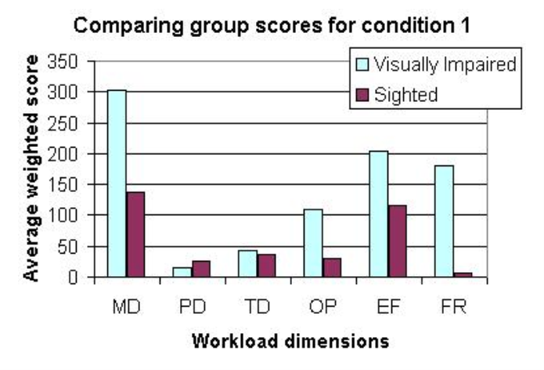
\includegraphics[width=\textwidth]{Revisao/Bradley Dunlop/Bradley Dunlop 2005 Nasa 3.png}
%        \caption{Condition 1.}
%        \label{fig:bradley_2005_nasa_participants_1}
%    \end{subfigure}
%    \hfill
%    \begin{subfigure}{.45\textwidth}
%        \centering
%        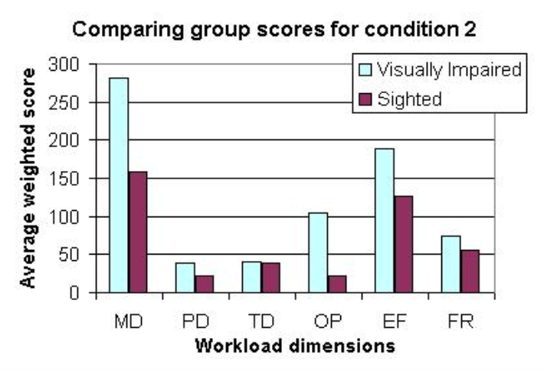
\includegraphics[width=\textwidth]{Revisao/Bradley Dunlop/Bradley Dunlop 2005 Nasa 4.png}
%        \caption{Condition 2.}
%        \label{fig:bradley_2005_nasa_participants_2}
%    \end{subfigure}
%\caption{Comparison of the NASA-TLX between the participants \cite{bradley2005experimental}.}
%\label{fig:bradley_2005_participants}
%\end{figure}


\FloatBarrier

This current experiment used their conclusion in order to create proper navigation commands used in the experiment. Another difference between this experiment and the one written by the duo is the inclusion haptics information in the scope of studied guidance commands.